\pgfplotsset{compat=1.17}

\section{Bloom Result}
\label{sec:BLOOM}
The task of this application is to minimize the value of metric "generation time per token" under the framework of Pytorch and Deepspeed. To simplify the meaning, we can describe it as : \\
\[\Phi_{token} = \frac{t_{gen} + t_{tokenize}}{n_{gen}}\]

In this formula, \(t_{gen}\) denotes the generation time required, \(t_{tokenize}\) signfies the tokenizing time required and \(n_{gen}\) represents the number of new token generated. Since the \(t_{tokenize}\) is far smaller than \(t_{gen}\), we can rewrite the equation as : \\
\[\Phi_{token} = \frac{t_{gen}}{n_{gen}}\]

To minimize the metric value for the BLOOM inference process, we can enhance the token inlet to generate more tokens, reduce the execution time, or implement both strategies.


\subsection{Batch size}
Our first strategy is to increase the total token inlet. By using Pytorch deep learning framework, we can easily transfer data from hosts to devices in pursue of better parallel ability.

Table~\ref{table:bloom-input} lists all sentences that will be fed as the input tokens. We found that the sentences will be duplicated several times in the list until the content in the list exceeds the batch\_size. Then, we will extract the first batch\_size sentences and feed them into the language model.

\begin{table}[t]
    \centering
    \caption{The input sentences for BLOOM inference}
    \label{table:bloom-input}
    \begin{tabular}{ll}
        \toprule
        Input\_sentences  \\
        \midrule
        "DeepSpeed is a machine learning framework" \\
        "He is working on" \\
        "He got all" \\
        "Everyone is happy and I can" \\
        "The new movie that got Oscar this year" \\
        "In the far far distance from our galaxy," \\
        "Peace is the only way" \\
        \bottomrule
    \end{tabular}
\end{table}

By experiments, we have found that the metric value decreases as we increasing the batch\_size as shown in Fig.~\ref{fig:exp_bloom_batch}.

\begin{figure}
\centering
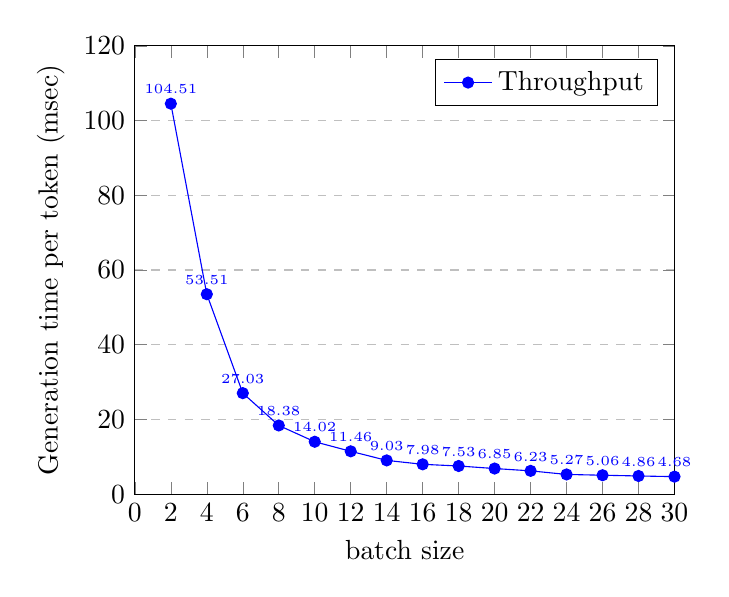
\begin{tikzpicture}
\begin{axis}[
    title={},
    xlabel={batch size},
    ylabel={Generation time per token (msec)},
    xmin=0, xmax=30,
    ymin=0, ymax=120,
    xtick={0,2,...,30},
    ytick={0,20,40,60,80,100,120},
    legend pos=north east,
    ymajorgrids=true,
    grid style=dashed,
    every node near coord/.append style={font=\tiny},
]

\addplot[
    color=blue,
    mark=*,
    nodes near coords,
    point meta=explicit symbolic, % Allows individual points to be labeled
    ]
    coordinates {
    (2,104.51) [104.51]
    (4,53.51) [53.51]
    (6,27.03) [27.03]
    (8,18.38) [18.38]
    (10,14.02) [14.02]
    (12,11.46) [11.46]
    (14,9.03) [9.03]
    (16,7.98) [7.98]
    (18,7.53) [7.53]
    (20,6.85) [6.85]
    (22,6.23) [6.23]
    (24,5.27) [5.27]
    (26,5.06) [5.06]
    (28,4.86) [4.86]
    (30,4.68) [4.68]
    };
    \legend{Throughput}

\end{axis}
\end{tikzpicture}
\caption{Generation time per token to batch size in two ASPIRE-2A A100x4 nodes}
\label{fig:exp_bloom_batch}
\end{figure}


\subsection{Deepspeed Optimization}
Here comes another strategy. The framework we choose for Bloom is Deepspeed. Developed by Microsoft, Deepspeed is an open-source deep learning optimization library specifically crafted to enhance the training efficiency and scalability of large deep learning models.

Deepspeed leverages tensor parallelism, a technique that distributes tensors across multiple GPUs. This method effectively breaks down a large model into numerous smaller segments, allocating them across various GPUs. Such a strategy enables models, which would typically exceed the capacity of a single GPU's memory, to be accommodated within multiple GPUs.

Moreover, as each GPU is assigned a segment of the overall computation, all GPUs are engaged in processing activities concurrently. Once they complete their individual computations, the GPUs exchange results through intercommunication, facilitating their progression to the next computational layer. By this approach, all the GPUs can work simultaneously, resulting in a better overall performance.

\subsection{NCCL Optimization}
Communication is another bottleneck of the execution time, here are some NCCL~\cite{jeaugey2017nccl} environment variables that we explored the best NCCL environment variables for running deepspeed inference on the Gadi supercomputer.
\subsubsection{NCCL\_NET\_GDR\_READ}
We set this variable to 1 (default 0 in non-NVlink based platform) to use GPU Direct RDMA to send data to the NIC directly.
\subsubsection{NCCL\_IB\_QPR\_PER\_CONNECTION}
We set this variable to "SYS" to always enable GPU Direct RDMA across nodes.
\subsubsection{NCCL\_NTHREADS}
By default, V100 on Gadi use 256 threads only. We set this variable to 512 to enlarge the CUDA threads per CUDA blocks. Increasing this variable can increase the GPU clock rate.
\subsubsection{NCCL\_BUFFSIZE}
This variable control the size of buffer used by NCCL when communicating between pairs of GPUs. By experiment, we have found that setting buffer size to 8Mb gives the best performance on Gadi.



\subsection{Comparison between Gadi and Taiwania2}
As depicted in Fig.~\ref{fig:exp_gadi_tw2}., despite of the batch size, Gadi consistently outperforms Taiwania 2. The speedup achieved on Gadi is more than 2 times faster.

We conducted Nsight System profiling, and observed that during the inference process, a significant portion of GPU kernel usage is dedicated to the ncclKernel allreduce operation, which is responsible for combining results. This highlights the communication demands between GPUs when employing Tensor Parallelism.

NCCL tests were conducted to evaluate the interconnection capabilities of both Gadi and Taiwania 2. The results indicate that Gadi has an impressive interconnection bandwidth of approximately 130 gigabytes per second, while Taiwania 2 has only about 12 gigabytes per second. This difference in interconnection bandwidth could indeed be one of the reasons why Gadi has a better performance. 

This insight highlights the importance of communication in large model inference.


\begin{figure}[h!]
\centering
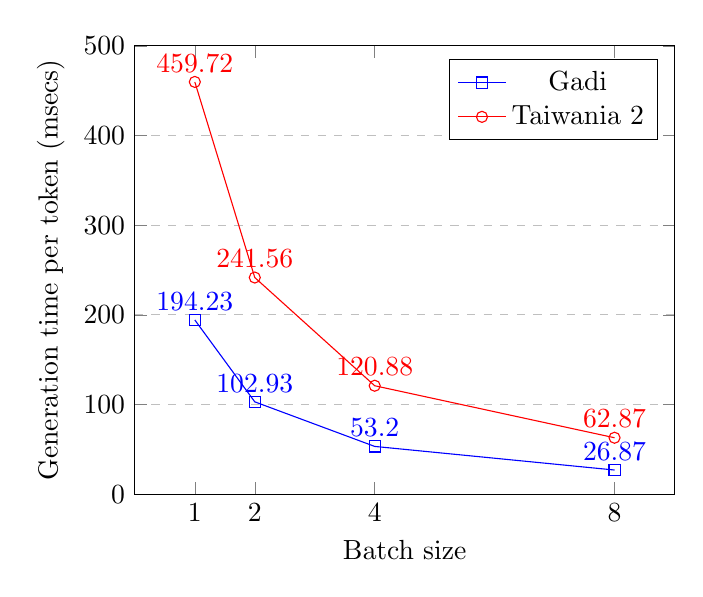
\begin{tikzpicture}
\begin{axis}[
    title={},
    xlabel={Batch size},
    ylabel={Generation time per token (msecs)},
    xmin=0, xmax=9,
    ymin=0, ymax=500,
    xtick={1,2,4,8},
    ytick={0,100,200,300,400,500},
    legend pos=north east,
    ymajorgrids=true,
    grid style=dashed,
    nodes near coords, % Enables data labels
]

% Gadi data
\addplot[
    color=blue,
    mark=square,
    ]
    coordinates {
    (1,194.23)(2,102.93)(4,53.2)(8,26.87)
    };
    \addlegendentry{Gadi}

% Taiwania 2 data
\addplot[
    color=red,
    mark=o,
    ]
    coordinates {
    (1,459.72)(2,241.56)(4,120.88)(8,62.87)
    };
    \addlegendentry{Taiwania 2}

\end{axis}
\end{tikzpicture}
\caption{Comparison of generation time per token for Gadi and Taiwania 2 across different batch sizes.}
\label{fig:exp_gadi_tw2}
\end{figure}


\subsection{Unsuccessful Attempts}
We've also tried to use some optimization tools provided by NVIDIA, but failed to achieve any significant improvement in our results, mostly due to memory issue.\\
Compared to deepspeed, which was the only method we successfully ran BLOOM-176B inference on Gadi and ASPIRE-2A, we concluded that it's because deepspeed provides one optimization -- Mixture of Quantization, which loads INT8 data and converts it to FP16 later when needed. This helps reduce the model size. \\
The following summarizes the optimization tools we've tried, why we tried, and why it failed.
\subsubsection{FasterTransformer} \cite{fastertransformer}
We've tried FasterTransformer since it claims that it provides some optimizations such as layer fusion, caching, support of multi-node, matmul kernel auto-tunning, etc.
However, it didn't have directly support of INT8 quantization for our BLOOM-176B model, which we thought would be unlikely to succeed. Therefore we turned to other tools after successfully building the required image.
\subsubsection{TensorRT} \cite{tensorrt}
We've also tried TensorRT, which we thought can make use of the TensortRT inference engine to improve the performance.
It first requires to convert BLOOM to ONNX format. With the former conclusion, any method without INT8 quantization might fail. Unfortunately, We are not allow to use other model (since the INT8 model provided seems to be only for deepspeed. Hence the only way we can do is to convert BLOOM-176B to ONNX first then do quantization. However, BLOOM-176B is such a large model that it's lots of work for us to transform the entire model. We make a pause after converting the first layer of BLOOM-176B.
\subsubsection{TensorRTLLM} \cite{tensorrt-llm}
Our last attempt was TensorRTLLM, which was just released recently. We thought it was the most suitable tool for us to use as its name showed. Not only it incorporates the desirable optimizations, such as kernel fusion, Tensor engine, ... some formally provided by FasterTransformer and TensorRT, it also provides python API and direct support of BLOOM-176B.
Though finding such powerful tool, we still fail to build TensorRT engine due to memory issue, as we encountered when using TensorRT.

To sum up, almost all the attempts failed due to insufficient memory, which is unsolvable. Therefore, although they provide many desirable optimizations, these tools are not feasible in our cases.